\documentclass{standalone}

\usepackage{tikz}
    
\usepackage{graphicx} % Работа с графикой \includegraphics{}
\graphicspath{{./images/img1/}} % картинки в папке ./images/img1/
    
\begin{document}

\begin{tikzpicture}
    \node at (-8.5,-2.5) 
        {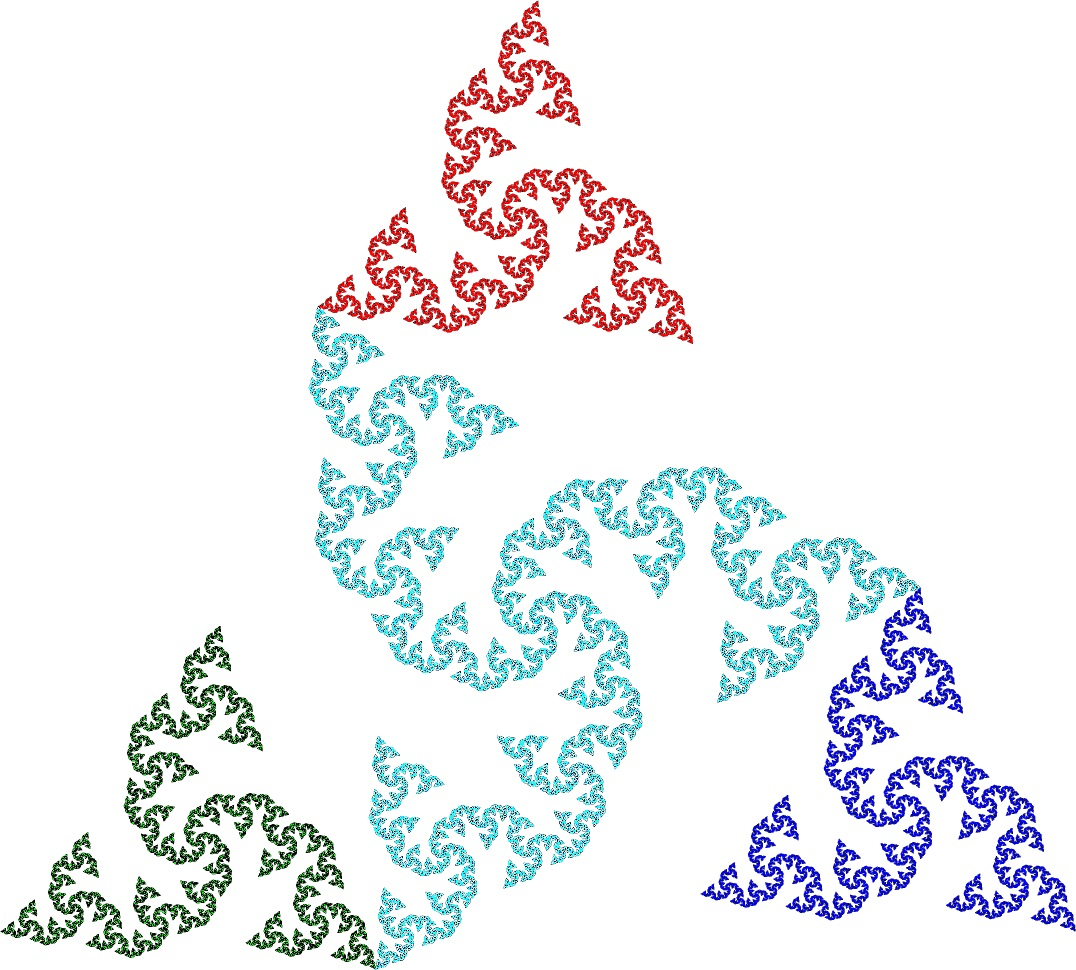
\includegraphics[width=4.76cm]{dirimage.jpg}};
    \node at (-2.5 ,-2.68) 
        {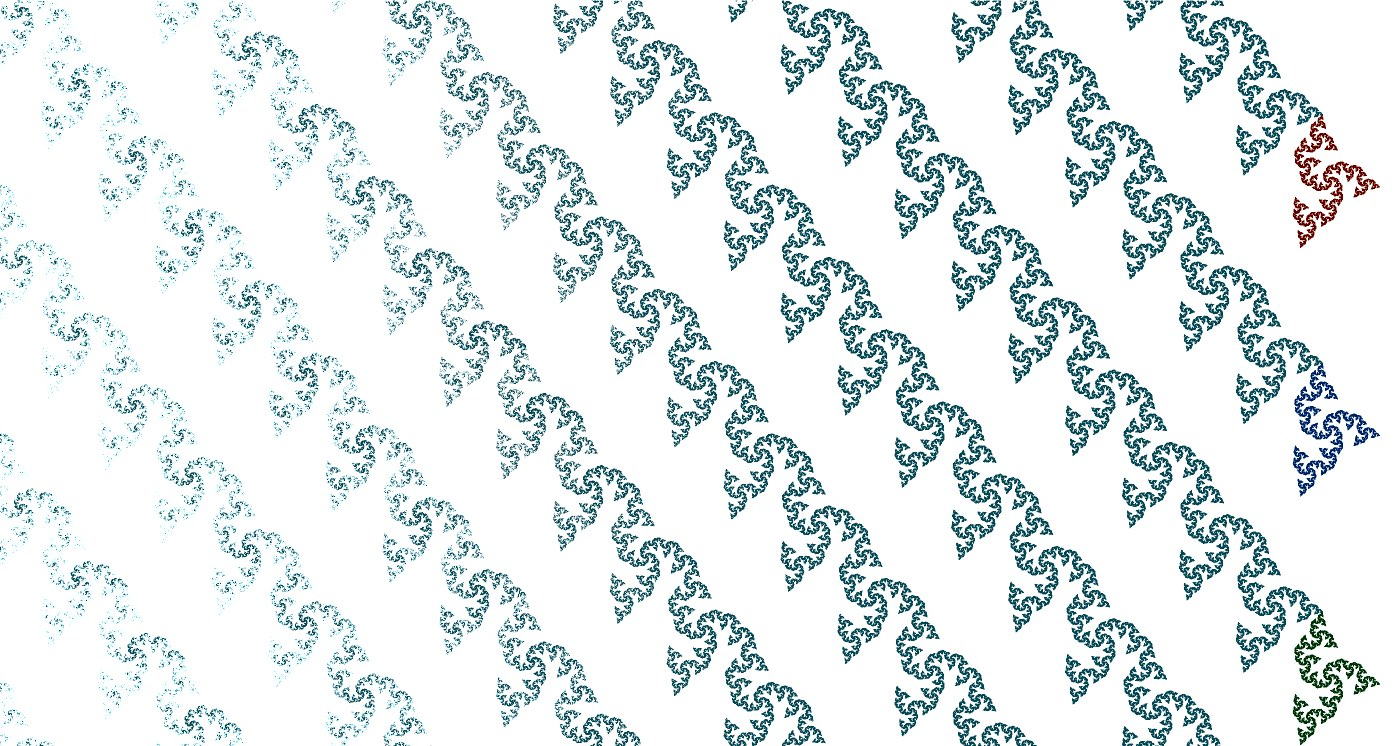
\includegraphics[width=5.95cm]{logimage3.jpg}};
    \node at (3.8,-2.68) 
        {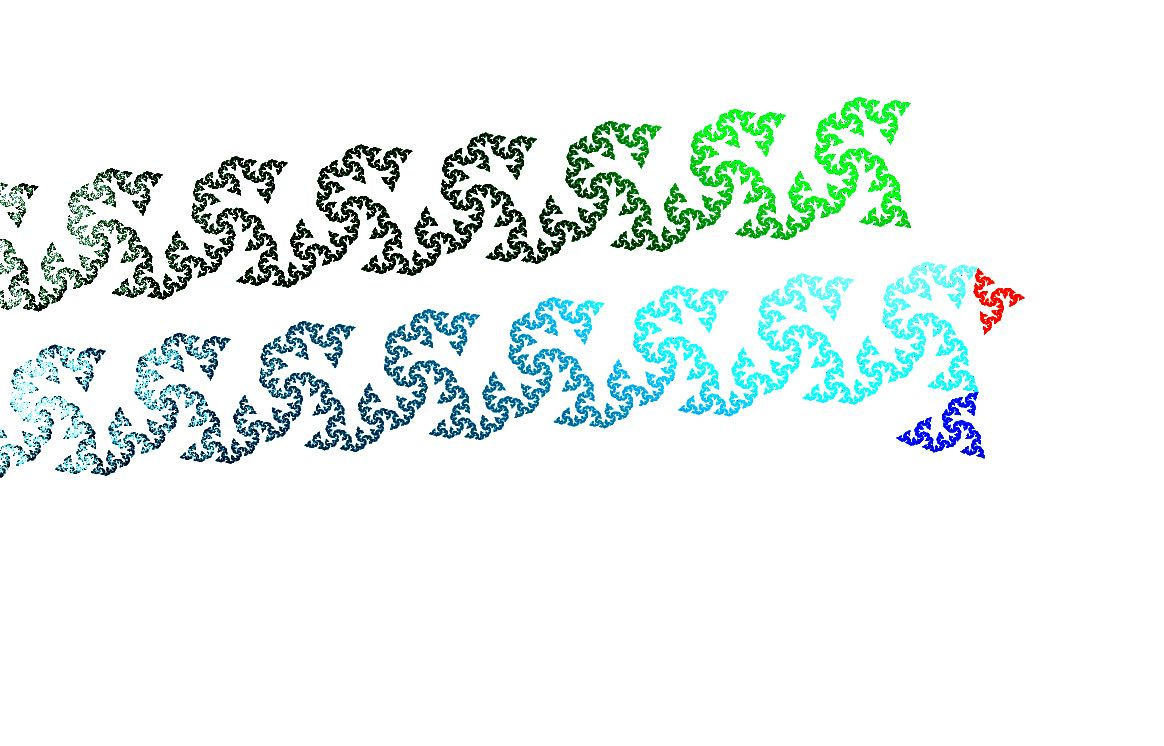
\includegraphics[width=5.95cm]{logimage2.jpg}};
    % \draw[step=.1,lightgray,ultra thin] (-11,-5) grid (6,0);
    % \draw[step=.2,yellow,ultra thin] (-11,-5) grid (6,0);
    % \draw[step=1,green, thin] (-11,-5) grid (6,0);
    \filldraw [fill=red]
        (-9.2,-4.67) circle (0.05) node[below] {$B$}
        (-8.5,-3.1)  circle (0.05) node[below] {$O$};
\end{tikzpicture}

\end{document}